\section{Meilenstein 3 $-$ Spezifikation, Implementierung
  und Demo eines REST-API}

% Teilaufgabe 1 {{{
\subsection{Teilaufgabe 1: Festlegen von Aggregates}%
\label{ms3_aggregates}

\begin{figure}[H]
\begin{center}
\begin{tikzpicture}

% Ebene 0 {{{
  \UMLClassAlterName
    {0}
    {0}
    {
      \textbf{Gericht}
        \nodepart{second}
      Name: String \\
      Details: String \\
      Preis: double
    }
    {gericht}
    {minimum width=6cm,text width=2.75cm,dashed}

  \UMLClassRelativeToAlterName
    {right=3 of gericht}
    {\textbf{Zutat}\nodepart{second}Name: String}
    {zutat}
    {minimum width=6cm}
% }}}

% Ebene -1 {{{
  \UMLClassRelativeToAlterName
    {below=3 of gericht}
    {\textbf{Speise}\nodepart{second}Name: String}
    {speise}
    {minimum width=6cm}
% }}}

% Ebene -2 {{{
  \UMLClassRelativeToAlterName
    {below=3 of speise}
    {
      \textbf{Zubereitungsanleitung}
        \nodepart{second}
      Anleitung: String
    }
    {za}
    {minimum width=6cm,fill=red!25}

  \UMLClassRelativeToAlterName
    {right=3 of za}
    {\textbf{Zutatenposition}\nodepart{second}Menge: int}
    {zutatenmenge}
    {minimum width=6cm,fill=red!25}
% }}}

% Verbindungen {{{
  % gericht -- speise {{{
  \draw[umlaggreg-] (gericht.south) -- (speise.north);
  \node[below left=.25 of gericht.south] {*};
  \node[above left=.25 of speise.north] {*};
  \node[left] at ($(gericht)!.5!(speise)$) {Teil von};
  % }}}
  % speise -- za {{{
  \draw[umlcompo-] (speise.south) -- (za.north);
  \node[below left=.25 of speise.south] {1};
  \node[above left=.25 of za.north] {1};
  \node[left] at ($(speise)!.5!(za)$) {beschreibt};
  % }}}
  % zutatenmenge -- za {{{
  \draw[-umlcompo] (zutatenmenge.west) -- (za.east);
  \node[above left=.25 of zutatenmenge.west] {1..*};
  \node[above right=.25 of za.east] {1};
  \node[below] at ($(zutatenmenge)!.5!(za)$) {ben\"otigt};
  % }}}
  % zutatenmenge -- zutat {{{
  \draw (zutatenmenge.north) -- (zutat.south);
  \node[above left=.25 of zutatenmenge.north] {*};
  \node[below left=.25 of zutat.south] {1};
  \node[left] at ($(zutatenmenge)!.5!(zutat)$) {ben\"otigt};
  % }}}
% }}}

% Aggregates {{{
\draw[rounded corners, red!75]
  ($(gericht.north) + (0,.5)$)
  --
  ($(gericht.north west) + (-.5,.5)$)
  |-
  ($(zutatenmenge.south east)+(.5,-.5)$)
  |-
  ($(gericht.north west) + (0,.5)$)
  --
  cycle
;
% }}}

\end{tikzpicture}
\end{center}
% Legende {{{
\tikz[baseline={-3pt}]{
  \node[fill=red!25,red!25,inner ysep=3pt]{X};
}: Value Object \\
\tikz[baseline={-3pt}]{
  \node[fill=yellow!25,yellow!25,inner ysep=2pt]{X};
}: Entity \\
\tikz[baseline={-3pt}]{
  \node[draw,red!75,inner ysep=3pt]{\textcolor{white}{X}};
}: Aggregate \\
\tikz[baseline={-3pt}]{
  \node[draw,dashed,inner ysep=3pt]{\textcolor{white}{X}};
}: Aggregate Root
% }}}
\caption{Aggregates}
\end{figure}


Wir sind der Meinung, dass sich die Datenobjekte Gericht,
Speise, Zubereitungsanleitung, Zutatenposition und Zutat
als ein Aggregate mit Gericht als Aggregate Root
zusammenfassen lassen, da keine Referenzen auf innere
Entities existieren und ein fachlicher Zusammenhang
besteht, da ein Gericht aus Speisen besteht, Speisen eine
Zubereitungsanleitung haben und diese wiederum
Zutatenpositionen, die auf Zutaten verweisen, ergibt sich
hier ein enges fachliches Geflecht. Au{\ss}erdem ist es so,
dass wir in Meilenstein 2 alle diese Objekte in der
Datenkomponente Gerichtsdaten (vgl. \ref{gos})
zusammengefasst haben, weshalb wir uns \"uberlegt haben,
dass das Aggregate durchaus deckungsgleich sein k\"onnte.

Eine m\"ogliche Invariante w\"are, wenn $Gericht.name$ eine
Kombination von den zugeh\"origen Speisen w\"are. Als
Beispiel hierf\"ur: $Gericht.name$: "`Schnitzel mit Pommes
und Salat"'. Daraus lassen sich die Speisen Schnitzel,
Pommes und Salat ableiten.
% }}}

% Teilaufgabe 2 {{{
\subsection{Teilaufgabe 2: Design des REST-API}

F\"ur unser REST-API verwenden wir folgenden Ausschnitt aus
unserem Klassendiagramm aus Meilenstein 1:

\begin{figure}[H]
\begin{center}
\begin{tikzpicture}

  \UMLClassAlterName
    {0}
    {0}
    {
      \textbf{Gericht}
        \nodepart{second}
      Name: String \\
      Details: String \\
      Preis: double
    }
    {gericht}
    {minimum width=6cm,text width=2.75cm, label=A/B}

  \UMLClassRelativeToAlterName
    {below=3 of gericht}
    {\textbf{Speise}\nodepart{second}Name: String}
    {speise}
    {minimum width=6cm,label={below:C}}

  \draw[umlaggreg-] (gericht.south) -- (speise.north);
  \node[below left=.25 of gericht.south] {*};
  \node[above left=.25 of speise.north] {*};
  \node[left] at ($(gericht)!.5!(speise)$) {Teil von};

\end{tikzpicture}
\end{center}
\caption{Ausschnitt Klassendiagramm f\"ur REST-API}
\end{figure}


\subsubsection*{Erl\"auterung}

Diese Schnittstelle w\"urde so in unserem Subsystem nicht
implementiert, da die verwendeten Gesch\"aftsobjekte nicht
in unser Subsystem geh\"oren und wir sie deshalb selbst
\"uber Schnittstellen aus anderen Subsystemen beziehen.
Wir bieten nur eine Schnittstelle f\"ur das
Gesch\"aftsobjekt Bestellung f\"ur die Buchhaltung an (vgl.
\ref{ms2_3}) und mit nur einem Gesch\"aftsobjekt l\"asst
sich das angegebene Szenario nicht durchf\"uhren, weshalb
wir den obrigen Ausschnitt verwenden.


\begin{tabu} to \linewidth {p{1.8cm}|X|p{2.5cm}|p{3cm}|X}
% Headerzeile {{{
\hline
\rowcolor{codebordercolor}
Szen.-Nr. &URI &HTTP Verb &Request-Body &Ressource und
  Aktion \\
% }}}
% A1, BC1, BC4, BC7 {{{
\hline
A1, BC1, BC4, BC7 &/gerichte &POST, GET
  &\textbf{Nur bei POST:}
    \{
      name=\dots,
      details=\dots,
      preis=\dots
    \}
  &Neues Gericht anlegen, alle Gerichte ausgeben. \\
% }}}
% A2, A4 {{{
\hline
A2, A4 &/gerichte?search= preis$>$\{wert\} &GET & &Alle
  Gerichte $a$ ausgeben, f\"ur die $a.preis > wert$ gilt.
  \\
% }}}
% A3 {{{
\hline
A3 &/gerichte/\{gericht\_id\}/ preis &PUT &\{wert\} &Preis
  von Gericht $a$ mit $a.gericht\_id=\{gericht\_id\}$ auf
  $\{wert\}$ setzen. \\
% }}}
% A6 {{{
\hline
A6 &/gerichte/\{gericht\_id\} &GET & &Ein bestimmtes
  Gericht \"uber die Id
  abfragen. 404 wird geworfen, falls Gericht nicht
  vorhanden. \\
% }}}
% BC2, BC5 {{{
\hline
BC2 &/speisen &POST, GET
  &\textbf{Nur bei POST:}
  \{name=\dots\}
  &Neue Speise anlegen. Alle Speisen ausgeben. \\
% }}}
% BC3, BC6 {{{
\hline
BC3, BC6 &/gerichte/\{gericht\_id\}/ speisen/\{speise\_id\}
  &PUT, DELETE & &Speise einem Gericht hinzuf\"ugen oder
  l\"oschen. \\
% }}}
\end{tabu}

\subsubsection*{Erl\"auterung}

Bei Szenario BC3 und BC6 haben wir uns entschieden, dass
die Beziehung zwsichen einer Instanz von Gericht und einer
Instanz von Speise \"uber /gerichte/\{gericht\_id\}/speisen
hinzugef\"ugt oder gel\"oscht weren kann. Man h\"atte dies
auch \"uber /speisen/\{speisen\_id\}/gerichte tun k\"onnen,
was wir jedoch f\"ur un\"ubersichtlicher und nicht so
naheliegend wie unsere Variante gehalten haben.

% }}}

\newpage

% Teilaufgabe 3 {{{
\subsection{Teilaufgabe 3: Implementierung in Spring Data
  JPA / Web MVC}

% Code-Listing {{{
\subsubsection{Code-Listing}

% GerichtRESTController {{{
\begin{mdframed}[style=codebox]
\textbf{GerichtRESTController}
\lstinputlisting[
  language=Java,
  firstline=34,
  lastline=152
]{%
  ../code/ms3RESTSpringDemo/src/main/java/%
  ms3restspringdemo/services/GerichtRestController%
  .java
}
\end{mdframed}
% }}}

% SpeiseRESTController {{{
\begin{mdframed}[style=codebox]
\textbf{SpeiseRESTController}
\lstinputlisting[
  language=Java,
  firstline=28,
  lastline=47
]
{%
  ../code/ms3RESTSpringDemo/src/main/java/%
  ms3restspringdemo/services/SpeiseRestController%
  .java
}
\end{mdframed}
% }}}

% }}}

% Custom JSON Serializer {{{
\subsubsection{Custom JSON Serializer}

%Vermeidung von Endlosschleifen bei der JSON-Ausgabe

Um das Problem der Endlosserialisierung bei der m:n-
Beziehung, die bei uns zwischen Gericht und Speise
vorliegt, zu l\"osen, wurde vorgeschlagen die Annotation
"`@JsonIdentityInfo"' zu benutzen, mit der man die
jeweiligen Klassen annotieren muss.

Die Serialisierung funktioniert dann so, dass beim ersten
Vorkommen einer Entit\"at diese ganz serialisiert wird,
beim zweiten Vorkommen allerdings nur über die ID
referenziert wird.

% {{{
\begin{mdframed}[style=codebox]
\textbf{Beispielausgabe der Gerichte}
\begin{lstlisting}
[
    {
        "id": 2,
        "name": "Schnitzel mit Pommes",
        "details": "Der grandiose Klassiker!",
        "preis": 12.5,
        "speisen": [
            {
                "id": 2,
                "name": "Schnitzel",
                "gerichte": [
                    2
                ],
            },
            {
                "id": 1,
                "name": "Pommes",
                "gerichte": [
                    2,
                    {
                        "id": 3,
                        "name": "Grosse Portion Pommes",
                        "details": "Lecker fettig!",
                        "preis": 6,
                        "speisen": [
                            1
                        ]
                    }
                ],
            }
        ]
    },
    3
]
\end{lstlisting}
\end{mdframed}
% }}}

Aus unserer Sicht ist die schlecht lesbare Ausgabe ein
Nachteil.

Ein Beispiel f\"ur die schlechte Lesbarkeit w\"are unserer
Meinung nach die "`3"' ganz unten (vorletzte Zeile, s.o.),
welche f\"ur das Gericht mit der ID 3 (Grosse Portion
Pommes) steht, welches bereits zuvor aufgef\"uhrt wurde.

Eine andere L\"osung, die wir gefunden haben ist ein
Custom-Serialisierer.

Hierbei k\"onnen wir dann selbst bestimmen, wie die
Serialisierung funktionieren soll.

Hier haben wir uns dafür entschieden nur einen
Serialisierer für die Gerichte, auf den die Speisen
verweisen, zu programmieren, der anstatt die Gerichte in
die "`Tiefe"' zu serialisieren, nur die IDs der Gerichte
auflistet. Damit w\"are dann das Endlosschleifen-Problem
gel\"ost.

Der Code dazu befindet sich in:
\begin{mdframed}[style=codebox]
\textbf{Relevanter Ausschnitt unseres Custom Serializers}
\lstinputlisting[language=Java, firstline=30]
{%
  ../code/ms3RESTSpringDemo/src/main/java/%
  ms3restspringdemo/serializers/CustomSetSerializer.java
}
\end{mdframed}

Um den Serializer für die Gerichte einzusetzen, muss eine
entsprechende Annotation mit dem Custom-Serialisierer bei
der Getter-Methode der Gerichte in der Klasse Speise
angebracht werden:

\begin{mdframed}[style=codebox]
\begin{lstlisting}
@JsonProperty
@JsonSerialize(using = CustomSetSerializer.class)
public Set<Gericht> getGerichte() {
	return Collections.unmodifiableSet(gerichte);
}
\end{lstlisting}
\end{mdframed}

% {{{
\begin{mdframed}[style=codebox]
\textbf{Beispielausgabe der Gerichte mit Custom Serializer}
\begin{lstlisting}
[
   {
      "id":2,
      "name":"Schnitzel mit Pommes",
      "details":"Der grandiose Klassiker!",
      "preis":12.5,
      "speisen":[
         {
            "id":2,
            "name":"Schnitzel",
            "gerichte":[
               2
            ]
         },
         {
            "id":1,
            "name":"Pommes",
            "gerichte":[
               3,
               2
            ]
         }
      ]
   },
   {
      "id":3,
      "name":"Grosse Portion Pommes",
      "details":"Lecker fettig!",
      "preis":6,
      "speisen":[
         {
            "id":1,
            "name":"Pommes",
            "gerichte":[
               3,
               2
            ]
         }
      ]
   }
]
\end{lstlisting}
\end{mdframed}
% }}}

Die Ausgabe ist, unserer Meinung nach, viel besser lesbar
und es ist einfacher mit ihr zu arbeiten.

Bei den Speisen sehen wir die Gerichte nun als eine Liste
von IDs.

Nachteil zu der vorigen L\"osung ist, dass Speisen mehrfach
aufgef\"uhrt werden, wie z.B "`Pommes"', weshalb die
Ausgabe mit dem Custom Serializer nicht redundanzfrei ist.

Trozdem ist unserer Meinung nach die Ausgabe des Custom
Serializers besser als die Ausgabe von
"`@JsonIdentityInfo"', da aus unserer Sicht eine wohl-
formatierte Ausgabe wichtiger ist als Redundanzfreiheit.
% }}}

\newpage

% Nachweis der Lauffaehigkeit {{{
\subsubsection{Nachweis der Lauff\"ahigkeit}

\begin{figure}[H]
  \begin{center}
    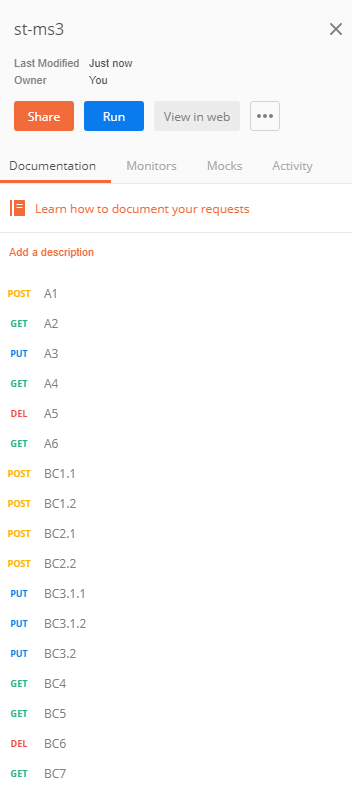
\includegraphics{ms3/static/postman_collection.PNG}
  \end{center}
  \caption{Postman Collection}
\end{figure}

\begin{figure}[H]
  \begin{center}
    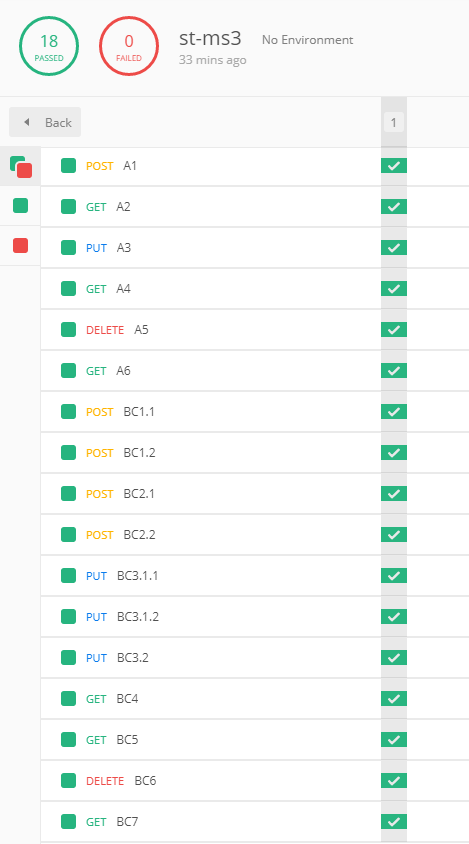
\includegraphics{ms3/static/postman_test.PNG}
  \end{center}
  \caption{Postman Test}
\end{figure}
% }}}

% }}}
